%%%%%%%%%%%%%%%%%%%%%%%%%%%%%%%%%%%%%%%%%%%%%%%%%%%%%%%%%%%%%%%%%%%%%%
% En 'setting.tex' se encuentran las configuraciones del proyecto
% En 'listings_settings.tex' se encuentran las configuraciones
% propias de listings, que es el paquete usado para incrustar código
%%%%%%%%%%%%%%%%%%%%%%%%%%%%%%%%%%%%%%%%%%%%%%%%%%%%%%%%%%%%%%%%%%%%%%
%%%%%%%%%%%%%%%%%%%%%%%%%%%%%%%%%%%%%%%%%
% University Assignment Title Page 
% LaTeX Template
% Version 1.0 (27/12/12)
%
% This template has been downloaded from:
% http://www.LaTeXTemplates.com
%
% Original author:
% WikiBooks (http://en.wikibooks.org/wiki/LaTeX/Title_Creation)
%
% License:
% CC BY-NC-SA 3.0 (http://creativecommons.org/licenses/by-nc-sa/3.0/)
% 
% Instructions for using this template:
% This title page is capable of being compiled as is. This is not useful for 
% including it in another document. To do this, you have two options: 
%
% 1) Copy/paste everything between \begin{document} and \end{document} 
% starting at \begin{titlepage} and paste this into another LaTeX file where you 
% want your title page.
% OR
% 2) Remove everything outside the \begin{titlepage} and \end{titlepage} and 
% move this file to the same directory as the LaTeX file you wish to add it to. 
% Then add \input{./title_page_1.tex} to your LaTeX file where you want your
% title page.
%
%%%%%%%%%%%%%%%%%%%%%%%%%%%%%%%%%%%%%%%%%
%\title{Title page with logo}
%----------------------------------------------------------------------------------------
%	PACKAGES AND OTHER DOCUMENT CONFIGURATIONS
%----------------------------------------------------------------------------------------
\documentclass[14pt]{extarticle}

%%%%%%%%%%%%%%%%%%%%%%%%%%%%%%%%%%%%%%%%%%%%%%%%%%
% En 'includes.tex' están todos los "\usepackage"
% (los "imports" de paquetes)
%%%%%%%%%%%%%%%%%%%%%%%%%%%%%%%%%%%%%%%%%%%%%%%%%%

%Paquetes para idioma español y codifcación UTF8
\usepackage[spanish]{babel}
\usepackage[utf8]{inputenc}
\usepackage{csquotes}

%%% BIBLATEX
\usepackage{biblatex}
%%% BIBLIOGRAPHY
\addbibresource{references.bib}

%paquete de matemática, vuela
\usepackage{amsmath}
%fuente 'fourier'
\usepackage{fourier}
%paquete para URLs
\usepackage{url}
%paquete para ubicar las imágenes
\usepackage{float}
%paquete para imágenes y en dónde las tiene que buscar
\usepackage{graphicx}
\graphicspath{{images/}}
%paquete para epígrafes
\usepackage{subcaption}
%paquete para definir los márgenes de la hoja
\usepackage[left=1.5cm,right=1.5cm,top=3cm,bottom=3cm]{geometry}
%paquete para poner todos y comentarios
\usepackage[colorinlistoftodos]{todonotes}
%paquete para trabajar con código
\usepackage{listings}
%paquete para trabajar con colores y definir propios
\usepackage{color}

%Cabeceras
\usepackage{fancyhdr}


\pagestyle{fancy}
\fancyhead[L]{Paradigmas de Lenguajes y Programación, 2018}
\fancyhead[C]{}
\fancyhead[R]{UNPSJB}

\fancyfoot[L]{SERRUYA ALOISI, TOLEDO MARGALEF}
\fancyfoot[R]{Laboratorio SMALLTALK}

%%paquete para reducir espacio entre secciones
%\usepackage{titlesec}
%\titlespacing*{\section}{0pt}{1.1\baselineskip}{\baselineskip}

%Comando para poner doble comillas más fácil
\newcommand{\dq}[1]{``#1''}

\definecolor{comment-green}{rgb}{0,0.5,0}
\definecolor{bg-light-gray}{HTML}{E9E9E9}
\definecolor{telegram-blue}{HTML}{148AC5}
\definecolor{keyword-alizarin}{rgb}{0.82, 0.1, 0.26}


% Sacado de
%https://gist.githubusercontent.com/mattonem/f434605a35716bfabec9/raw/7725cdbdf2424b2c81f91a96324bfdb54efa626f/smalltalkEnv.tex
\lstdefinelanguage{smalltalk}{
  keywordstyle=\color{stKeywords}\ttfamily,
  commentstyle=\color{stComment}\ttfamily,
  stringstyle=\color{stString}\ttfamily,
  alsoletter=\#,
  identifierstyle=\ttfamily, 
  showstringspaces=false,
  morekeywords={true,false,self,super,nil},
  sensitive=true, 
  morecomment=[s]{"}{"}, 
  tabsize=2,
}

\lstdefinestyle{smalltalk}{
    language=smalltalk,
    backgroundcolor=\color{bg-light-gray},
  	keywordstyle=\bfseries\color{keyword-alizarin}\ttfamily,
    stringstyle=\color{telegram-blue}\ttfamily,
    commentstyle=\color{comment-green}\itshape\ttfamily,
    numberstyle=\color{gray}\ttfamily,
    identifierstyle=\color{black}\ttfamily,
    rulecolor=\color{gray},
    showstringspaces=false,
    escapeinside={\%*}{*)},
  	morekeywords={TipoCliente,TipoBebida},
    otherkeywords={::,=,==,not,++},
    breaklines=true,
  	title=\lstname,	
    frame=trbl, 
    framexleftmargin=25pt,
    numbers=left,
    xleftmargin=\parindent,
    frameround=tttt,
    % re tirado de los pelos, pero es lo que hay
    % sacado de:
    % https://tex.stackexchange.com/questions/24528/having-problems-with-listings-and-utf-8-can-it-be-fixed
    inputencoding=utf8,
    extendedchars=true,
    literate={á}{{\'a}}1 {é}{{\'e}}1 {í}{{\'i}}1 {ó}{{\'o}}1 {ú}{{\'u}}1,
}

%\input{smalltalk_listings_settings}


\begin{document}

%%%%%%%%%%%%%%%%%%%%%%%%%%%%%%%%%%%%%%%%%%%%
% En 'titlepage.tex' se encuentra la página de título
%%%%%%%%%%%%%%%%%%%%%%%%%%%%%%%%%%%%%%%%%%%%
\begin{titlepage}

    \newcommand{\HRule}{\rule{\linewidth}{0.5mm}} % Defines a new command for the horizontal lines, change thickness here

    \center % Center everything on the page
     
    %----------------------------------------------------------------------------------------
    %	HEADING SECTIONS
    %----------------------------------------------------------------------------------------

    \textsc{\LARGE UNPSJB}\\[1cm] % Name of your university/college
    \textsc{\Large Licenciatura en Sistemas OPGCPI}\\[0.5cm] % Major heading such as course name
    \textsc{\large Paradigmas de Lenguajes y Programación}\\[0.5cm] % Minor heading such as course title

    %----------------------------------------------------------------------------------------
    %	TITLE SECTION
    %----------------------------------------------------------------------------------------

    \HRule \\[0.4cm]
    {\huge \bfseries Paradigma objetos}\\[0.4cm] % Title of your document
    {\large \bfseries Laboratorio SMALLTALK}\\[0.4cm] % Title of your document
    \HRule \\[1.5cm]
     
    %----------------------------------------------------------------------------------------
    %	AUTHOR SECTION
    %----------------------------------------------------------------------------------------


    \begin{minipage}[l]{0.5\textwidth}
        \begin{flushleft}
            \textbf{\textsf{Cátedra}}\\
            \large Lic. Romina Stickar\\ 
            \large Lic. Lautaro Pecile\\ 
            \linespread{4}
            \end{flushleft}
    \end{minipage}
    \begin{minipage}[l]{0.4\textwidth}
        \begin{flushright}
            \textbf{\textsf{Integrantes:}}\\
            \linespread{1}
            \large Luciano Serruya Aloisi\\
            \large Pablo Toledo Margalef\\
        \end{flushright}
    \end{minipage}\\[1.5cm]

    % If you don't want a supervisor, uncomment the two lines below and remove the section above
    %\Large \emph{Author:}\\
    %John \textsc{Smith}\\[3cm] % Your name

    %----------------------------------------------------------------------------------------
    %	DATE SECTION
    %----------------------------------------------------------------------------------------

    {\large \today}\\[1cm] % Date, change the \today to a set date if you want to be precise

    %----------------------------------------------------------------------------------------
    %	LOGO SECTION
    %----------------------------------------------------------------------------------------

    
\includegraphics[scale=1]{logoUnpsjb.png}\\[0.5cm] % Include a department/university logo - this will require the graphicx package
     
    %----------------------------------------------------------------------------------------

    % \vfill % Fill the rest of the page with whitespace

\end{titlepage}


%%%%%%%%%%%%%%%%%%%%%%%%%%%%%%%%%%%%%%%%%%%%
% INDICE
%%%%%%%%%%%%%%%%%%%%%%%%%%%%%%%%%%%%%%%%%%%%
\clearpage
\tableofcontents
\clearpage 
%%%%%%%%%%%%%%%%%%%%%%%%%%%%%%%%%%%%%%%%%%%%
% ABSTRACT
%%%%%%%%%%%%%%%%%%%%%%%%%%%%%%%%%%%%%%%%%%%%
%\begin{abstract}
%Your abstract.
%\end{abstract}

\lstset{style=smalltalk}

\section{Modelado del dominio}

El dominio de la aplicación consta de \textbf{unidades}, \textbf{tanques}, y \textbf{misiles}. 

\subsection{Clases}

\subsubsection{Unidad}

Una unidad consta de un nombre y de varios tanques de distinto tipo. Saben devolver y cambiar su nombre en tiempo de ejecución, devolver todos sus tanques, o solamente aquellos que están vivos (un tanque está vivo si tiene munición, tripulantes y coraza). También pueden hacer que todos sus tanques se muevan a una misma velocidad.

Los tanques se pueden atacar entre sí, y para ello las unidades tienen la capacidad de indicar a sus tanques que ataquen a tanques de una unidad dada

\subsubsection{Tanque}

La clase central de la aplicación es el tanque. 

Al igual que la unidad tienen un nombre; como ya se dio a conocer, los tanques tienen tripulantes, coraza, una velocidad de movimiento, y una munición.

Cada tanque sabe cómo atacar a otro tanque (obtienen un misil aleatorio de su arsenal y le infligen el daño correspondiente). Pueden hacer un reconocimiento de su estado, en cuanto a si tienen o no munición, tripulantes, si está en movimiento, si emite calor (un tanque emite calor si se está moviendo o si tiene más de tres tripulantes), si puede disparar (en movimiento o no), o si está vivo siquiera. Un tanque reconoce cuando un impacto de misil es un \emph{golpe fuerte} (valor de daño mayor a 50); en tal caso, muere uno de sus tripulantes.

Existen distintos tipos de tanques, cada uno con distintos valores posibles de munición, coraza, cantidad de tripulantes o velocidad máxima. Ellos son:

\begin{itemize}
    \item Tanque rápido
    \item Tanque liviano
    \item Tanque pesado
    \item Tanque dron
    \item Tanque con blindaje electromagnético (\emph{EM})
\end{itemize}

Al momento de que un tanque ataque a otro, se toman en cuenta las velocidades de movimiento tanto del tanque atacante como la del atacado. Cada uno de los distintos tipos de tanques reacciona diferente frente al impacto de un misil; particularmente el \emph{tanque dron} no tiene perdida de daño por precisión, y el \emph{tanque EM} recibe solamente 80\% del daño causado.

%Cuando un tanque ataca a una unidad, se vale del mensaje que tienen las unidades para devolver uno de sus tanques vivos

\subsubsection{Misil}

La munición que tiene un tanque determina la cantidad de misiles disponibles en su arsenal.

El daño que le hará un misil a un tanque dependerá tanto del tipo de tanque que sea y su estado actual, como del tipo de misil lanzado. 

La \emph{Bazooka} y el \emph{Misil Groso} tienen pérdida de daño por precisión (2 y 3 puntos cada 5 KM/H, respectivamente). Este valor afectará en el cálculo del daño total a inflingir sobre el tanque atacado. 

Los puntos de impacto de una \emph{Bazooka} serán el doble de las \emph{cabezas nucleares} que tenga (a lo sumo 4).  

El \emph{Misil térmico} únicamente impactará contra los tanques que emitan calor, sin tener en cuenta las velocidades de los tanques involucrados en el ataque. Estos misiles tienen la particularidad de que se puede cambiar cuántos puntos de impacto realizan sobre un tanque en tiempo de ejecución.

\subsubsection{Escenario}

Uno de los requisitos de la aplicaión era implementar un funcionalidad para que, dadas dos unidades, se ataquen mutuamente hasta que alguna de las dos quede sin tanques vivos. Para ello se debió considerar un \textbf{Escenario} que tenga todas las unidades presentes en la simulación. Existirá un único escenario que tenga todas las unidades, pudiendo pedírselas o agregarle nuevas.

\subsection{Diseño}

\subsubsection{Diagrama de clases}

Para modelar los requerimientos previamente descriptos, se diseñó el siguiente \emph{diagrama de clases software} 

\begin{figure}[H]
    \centering
    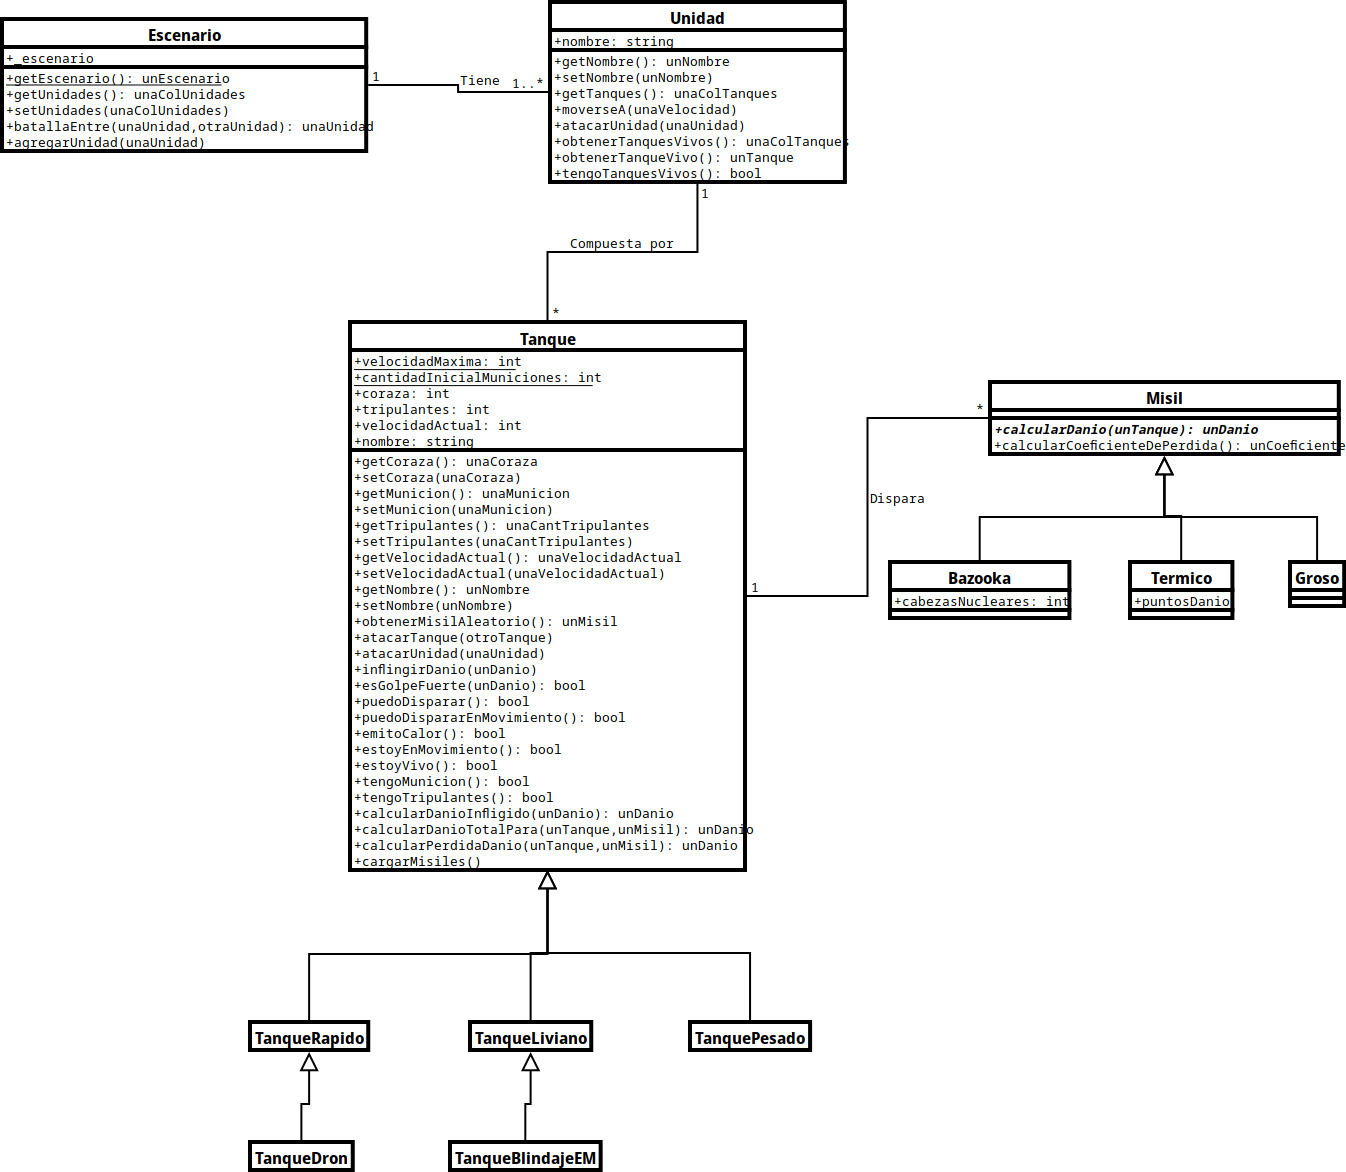
\includegraphics[width=\textwidth, height=\textheight-15pt]{clases.png}
    \caption{Escenario, Unidad, Tanque, y Misil}
\end{figure}

\subsubsection{Interacción entre objetos}

El siguiente \emph{diagrama de secuencia de objetos} modela resumidamente cómo es la comunicación entre objetos en tiempo de ejecución al momento enviarle el mensaje 

{\ttfamily atacarTanque: unTanque} a un tanque. 

\begin{figure}[H]
    \centering
    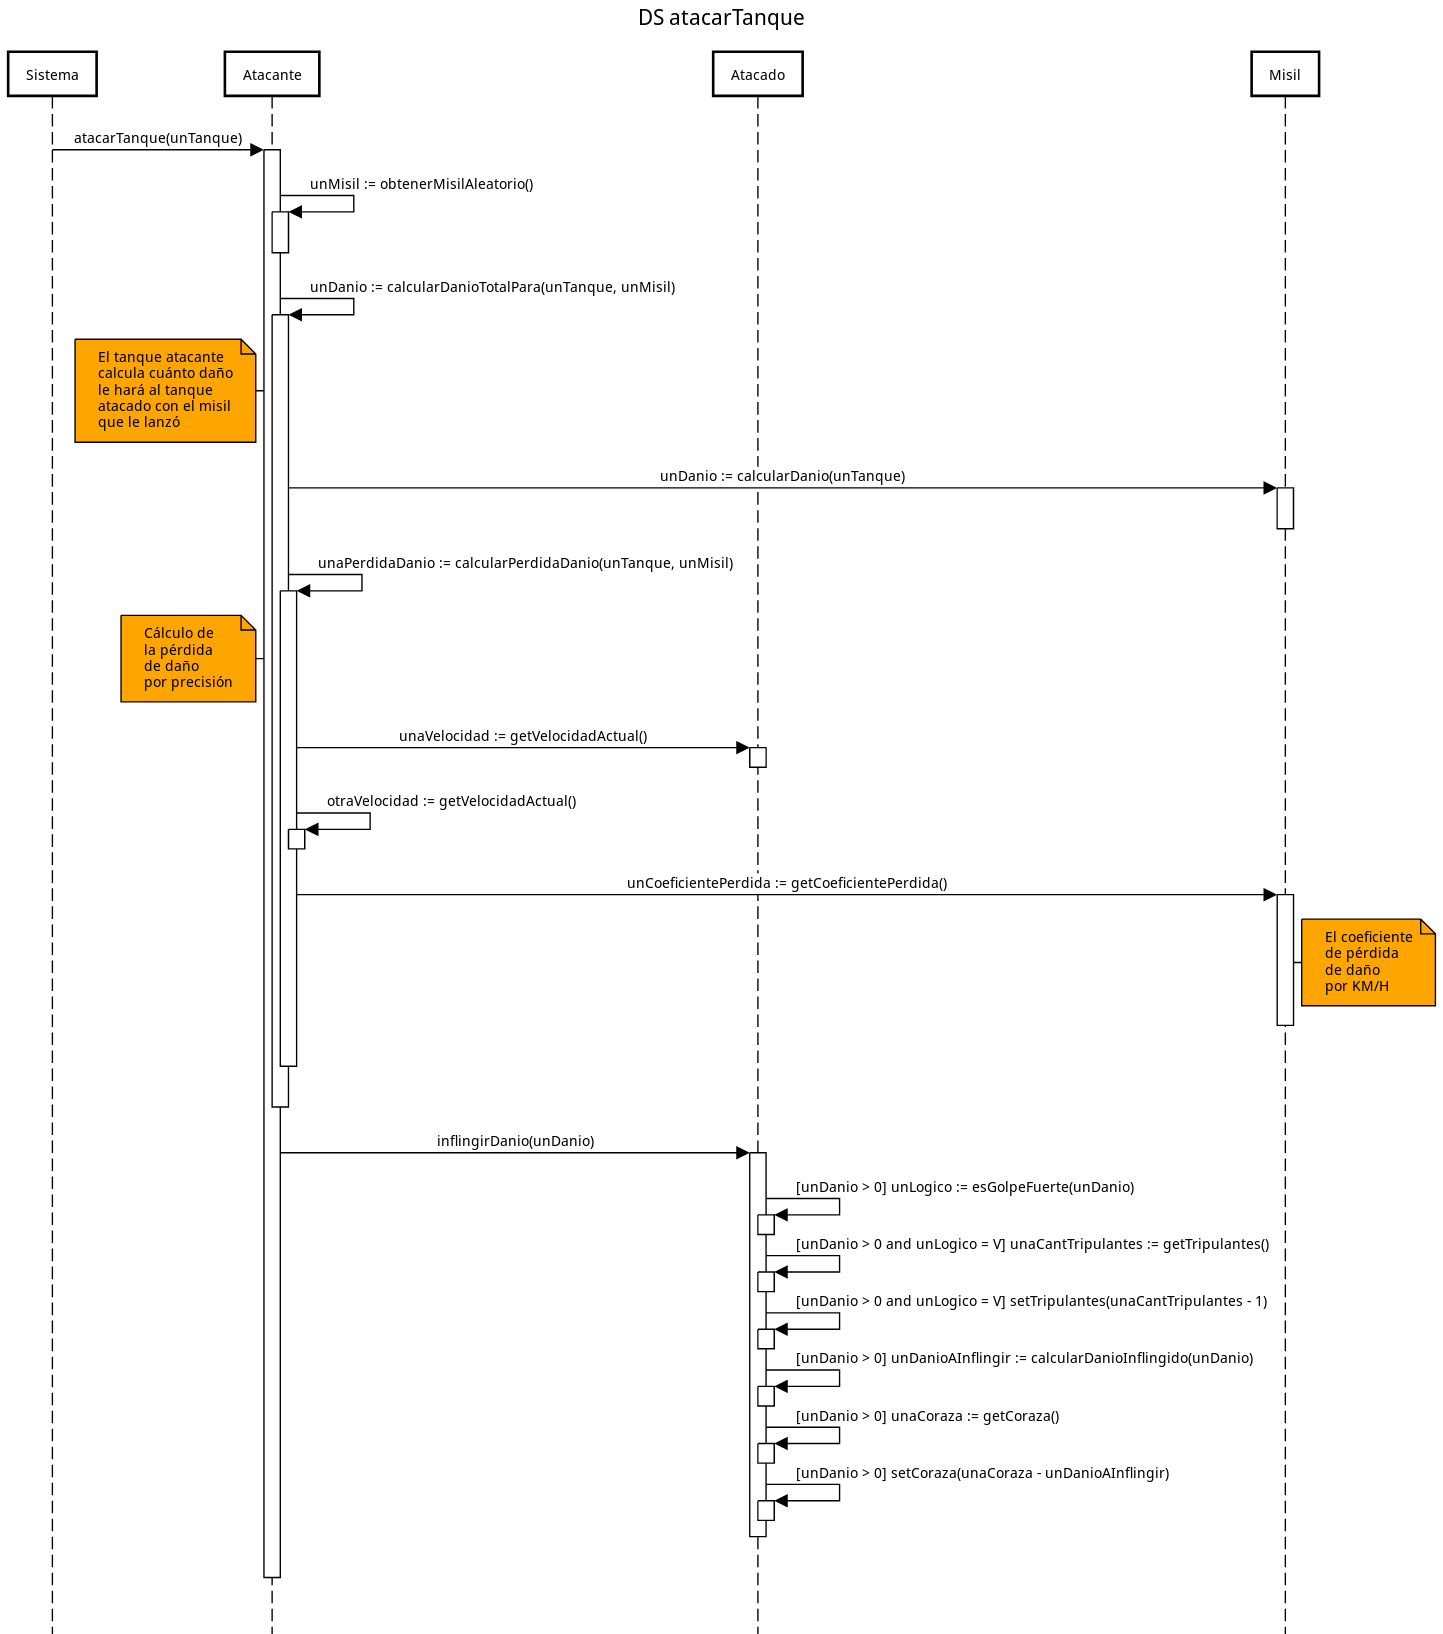
\includegraphics[width=\textwidth, height=\textheight-25pt]{ds_atacarTanque.png}
    \caption{Diagrama de secuencia de {\ttfamily unTanque atacarTanque: otroTanque} (realizado con \autocite{ds})}
\end{figure}

Nótese que el diagrama anterior no considera comportamientos particulares del tanque ni del misil, solamente ilustra generalmente el intercambio de mensajes entre los objetos que intervienen.




\subsubsection{Patrones implementados}

Un \emph{Patrón de Diseño} es definido en \autocite{gof} como \emph{descripciones de clases y objetos relacionados que están particularizados para resolver un problema de diseño general en un determinado contexto}. También se los clasifica en tres grandes grupos: \textbf{de creación}, \textbf{de comportamiento}, y \textbf{de estructura}.    

El primer patrón implementado en el diseño de las clases se lo clasifica como un patrón comportamiento de clase, y es el patrón \textbf{Template Method} ó \textbf{Plantilla}. Su implementación se puede ver en los mensajes {\ttfamily calcularDanioInflingido} de la clase \emph{Tanque}, y en {\ttfamily calcularDanio} de \emph{Misil}.

Por otro lado, la clase \emph{Escenario} implementa el patrón de creación \textbf{Singleton}, que consiste en tener una clase con una única instancia (se accede a través de un método de clase). El método de clase para acceder al escenario es {\ttfamily getEscenario}

\section{Simulación}

Para correr la simulación, cargar el paquete {\ttfamily TP-Tanque.st} al entorno de \emph{Pharo}, luego abrir el \emph{Workspace} (ambos archivos se pueden encontrar en el directorio \emph{src/}) y ejecutar las sentencias.  




%%%%%%%%%%%%%%%%%%%%%%%%%%%%%%%%%%%%%%%%%%%%
% FIN DOCUMENTO, AHORA REFERENCIAS
%%%%%%%%%%%%%%%%%%%%%%%%%%%%%%%%%%%%%%%%%%%%
\clearpage
\printbibliography

\end{document}
\todo[inline, color=green!40]{This is an inline comment.}

\subsection{}
\emph{} 

~\\

\begin{lstlisting}
 girlInBar phoneNumber 
        jerk say: 'Get lost'
        jerk throwAt: drink
        self leave: bar
        ^ '1-800-GET-LOST'
\end{lstlisting}
